\documentclass[dvisvgm,tikz,border=4pt]{standalone}
\usepackage{amsmath,amssymb}

\usetikzlibrary{arrows.meta,positioning,automata,shapes,shapes.misc,calc,decorations.pathmorphing,decorations.markings,angles,quotes,patterns,mindmap,matrix,knots,hobby,trees}
\tikzset{->-/.style={decoration={markings, mark=at position 0.5 with {\arrow{Stealth}}}, postaction={decorate}}}
\begin{document}
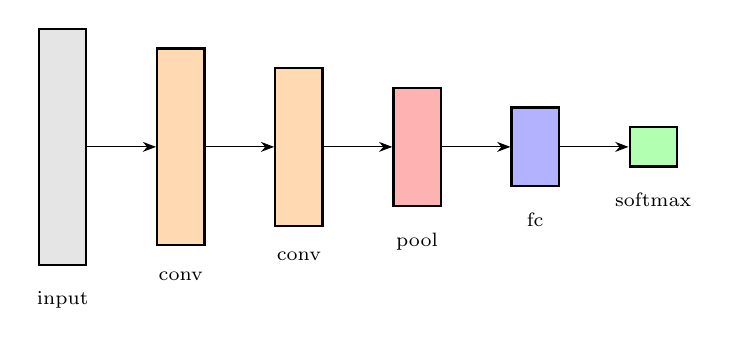
\begin{tikzpicture}[box/.style={draw, thick, minimum height=#1, minimum width=6mm, fill=orange!30}, >=Stealth]
\node[box=3cm, fill=gray!20] (in) at (0,0) {};
\node[box=2.5cm] (c1) at (1.5,0) {}; \node[box=2cm] (c2) at (3,0) {}; \node[box=1.5cm, fill=red!30] (p) at (4.5,0) {};
\node[box=1cm, fill=blue!30] (f) at (6,0) {}; \node[box=5mm, fill=green!30] (o) at (7.5,0) {};
\foreach \a/\b in {in/c1, c1/c2, c2/p, p/f, f/o} \draw[->] (\a) -- (\b);
\foreach \n/\l in {in/input, c1/conv, c2/conv, p/pool, f/fc, o/softmax} \node[below=2mm of \n, font=\scriptsize] {\l};
\end{tikzpicture}
\end{document}
